\RequirePackage[l2tabu, orthodox]{nag}
\documentclass[version=3.21, pagesize, twoside=off, bibliography=totoc, DIV=calc, fontsize=12pt, a4paper]{scrartcl}
\input{preamble/packages}
\input{preamble/redac}
\input{preamble/math_basics}
%Pref
\NewDocumentCommand{\pref}{O{}}{⊳^{#1}}
\NewDocumentCommand{\prefeq}{O{}}{⊵^{#1}}
\NewDocumentCommand{\prefinv}{O{}}{⊲^{#1}}
\NewDocumentCommand{\prefeqinv}{O{}}{⊴^{#1}}
\NewDocumentCommand{\ppref}{}{\succ}
\NewDocumentCommand{\pprefeq}{}{\succeq}
\NewDocumentCommand{\pprefinv}{}{\prec}
\NewDocumentCommand{\pprefeqinv}{}{\preceq}
\NewDocumentCommand{\upb}{O{b}}{{\uparrow}#1}
\NewDocumentCommand{\downb}{O{b}}{{\downarrow}#1}
\NewDocumentCommand{\POs}{O{X}}{\mathit{PO}(#1)}

%Prob
\NewDocumentCommand{\inQ}{}{\intvl{1, \card{Q}}}
%Decision Theory (MCDA and SC)
\NewDocumentCommand{\allalts}{}{X}
\NewDocumentCommand{\allcrits}{}{\mathscr{C}}
\NewDocumentCommand{\alts}{}{A}
\NewDocumentCommand{\dm}{}{i}
\NewDocumentCommand{\allF}{}{\mathscr{F}}
\NewDocumentCommand{\allvoters}{}{\mathscr{N}}
\NewDocumentCommand{\voters}{}{N}
\NewDocumentCommand{\allprofs}{}{\bm{\mathcal{R}}}
\NewDocumentCommand{\prof}{}{\bm{R}}
\NewDocumentCommand{\linors}{O{X}}{\mathscr{L}(#1)}
%Thanks to https://tex.stackexchange.com/q/154549
	%\makeatletter
	%\def\@myRgood@#1#2{\mathrel{R^X_{#2}}}
	%\def\myRgood{\@ifnextchar_{\@myRgood@}{\mathrel{R^X}}}
	%\makeatother

%Deliberated Judgment
\NewDocumentCommand{\allargs}{}{S^*}
\NewDocumentCommand{\args}{}{S}
\NewDocumentCommand{\ar}{}{s}
\NewDocumentCommand{\allprops}{}{T}
\NewDocumentCommand{\prop}{}{t}
\NewDocumentCommand{\ileadsto}{}{⇝}
\NewDocumentCommand{\ibeatse}{}{⊳_\exists}
\NewDocumentCommand{\nibeatse}{}{⋫_\exists}
\NewDocumentCommand{\ibeatsst}{}{⊳_\forall}
\NewDocumentCommand{\nibeatsst}{}{⋫_\forall}
\NewDocumentCommand{\mleadsto}{O{\eta}}{⇝_{#1}}
\NewDocumentCommand{\mbeats}{O{\eta}}{⊳_{#1}}
\NewDocumentCommand{\ibeatseinv}{}{⊳_\exists^{-1}}

%Logic
\NewDocumentCommand{\ltru}{}{\texttt{T}}
\NewDocumentCommand{\lfal}{}{\texttt{F}}

\NewDocumentCommand{\relq}{}{\mathrel{?}}


\newcommand{\commentMP}[1]{\textcolor{green}{[MP:#1]}}
%I find these settings useful in draft mode. Should be removed for final versions.
	%Which line breaks are chosen: accept worse lines, therefore reducing risk of overfull lines. Default = 200.
		\tolerance=2000
	%Accept overfull hbox up to...
		\hfuzz=2cm
	%Reduces verbosity about the bad line breaks.
		\hbadness 5000
	%Reduces verbosity about the underful vboxes.
		\vbadness=1300

\title{Probabilistic elicitation of preferences \thanks{Draft!}}
\author{Nicolas Boria}
\author{Olivier Cailloux}
\author{Ararat Harutyunyan}
\affil{Université Paris-Dauphine, PSL Research University, CNRS, LAMSADE, 75016 PARIS, FRANCE\\
	\href{mailto:olivier.cailloux@dauphine.fr}{olivier.cailloux@dauphine.fr}
}

\begin{document}
\maketitle

\section{Set up and goal}
\begin{itemize}
	\item $\allalts$ a set of objects. Example: $\allalts = {a, b, c}$.
	\item $n = |\allalts|$. Example: $n = 3$.
	\item $\linors$ the set of linear orders over $\allalts$, that is, of transitive, connected and irreflexive binary relations over $\allalts$ (a relation $>$ over $\allalts$ is connected iff $\forall i ≠ j \in \allalts: i > j \lor j > i$). 
	\item ${>} \in \linors$ a preference over $\allalts$. Example: $\set{(a, b), (a, c), (b, c)}$.
\end{itemize}
The preference $>$ is unknown a priori, and we will ask random questions to obtain information about it. We only know the probability distribution over $\linors$, from which $>$ is drawn. We are interested in evaluating the probabilistic evolution of our knowledge of $>$ as a function of the number of questions asked. 

\section{Questioning to increase our knowledge}
$E \subseteq \allalts × \allalts$: a set of oriented edges \commentMP{``directed edges'' or ``arcs''}. It represents our knowledge of $>$.
The possible sets of edges are all $E$ that are transitive and acyclic. \commentMP{Il faut décider si on travaille avec des relations réflexives ou irréflexives; distinguer aussi les graphes orientés des non-orientés; adopter une terminologie non-ambigüe)}
We can think of $E$ as a \commentMP{directed graph or digraph} graph whose set of nodes is $\allalts$. We thus define a bijection that relates $E$ to $G = (\allalts, E)$, its corresponding graph, and talk interchangeably about a graph or a set of edges. This defines the possible graphs: those having nodes $\allalts$ and a transitive and acyclic set of edges.

Let $E_t$ denote our knowledge after $t$ questions.
Define $E_0 = \emptyset$ as our (empty) knowledge after zero questions.
Example of $E_1 : \set{(a, b)}$.

A question $q \in Q$ is a non-oriented edge, which formally we consider as two edges, inverse of each other. Let $q_{ij} = \set{(i, j), (j, i)}$ denote the question about ${i, j}$, with $i ≠ j \in \allalts$.
Note that $q_{ij} = q_{ji}$.
The set of possible questions is $Q = \set{q_{ij} \suchthat i ≠ j \in \allalts}$.
It follows that $\card{Q} = \frac{n (n - 1)}{2}$. In our running example, $\card{Q} = 3$.

Given $i ≠ j \in \allalts$, let $q_{ij}(>)$ represent, intuitively, the answer to the question $q_{ij}$ when the preference is $>$, that is, $q_{ij}(>)$ is the edge connecting $\set{i, j}$ that is in $>$, or formally, the element of the singleton ${>} \cap q_{ij}$.
Define an addition operation over the possible graphs, representing our increase in knowledge after having obtained an answer to a question: we add the resulting edge, and compute the transitive closure. Formally, given $E$ and a question $q$, $E + q(>) = T(E \cup \set{q(>)})$, where $T$ denotes the irreflexive transitive closure. Example: $\set{(a, b)} + q_{bc}(>) = {>}$.

Let $K_E = \set{\set{e, e^{-1}} \suchthat e \in E} \subseteq Q$ denote the questions whose answer is known in $E$. Note that $\card{K_E} = \card{E}$.
Let $Q_E = Q \setminus K_E$ denote the questions remaining given $E$. Note that $\card{Q_E} = \card{Q} - \card{K_E}$.
Note that if we obtain at least one edge per step, then after $\card{Q}$ steps, our knowledge is complete: $Q_{E_{\card{Q}}} = 0$.

\section{The probability distribution of interest}
Let $\powerset{S}$ denote the set of subsets of $S$.
Let $P: \powerset{\linors × Q^{\card{Q}}} → [0, 1]$ denote the probability distribution over the possible preferences and questions asked. Thus, if $\card{Q} = 3$, $P(>, q_1, q_2, q_3)$ denotes the probability that the preference is $>$ and that the questions asked were $q_1$, then $q_2$, and finally $q_3$.

Let $\inQ$ denote the interval of integers between $1$ and $\card{Q}$.
Let $P(\set{(>, (E_t)_{t \in \inQ})}) = P(\set{(>, (q_t)_{t \in \inQ}) \suchthat \forall t \in \inQ: E_t = E_{t - 1} + q_t})$ denote the probability that the preference is $>$ and that the questions asked lead to the sequence of graphs $(E_t)_{t \in \inQ}$.
Example: $P(E_1 = \set{(a, b)}) = P(q_1 = q_{ab})$.
Example: $P(E_2 = \set{(a, b), (c, b)}) = P\big((\set{q_1, q_2} = \set{q_{ab}, q_{bc}}) \text{ and } a > b \text{ and } c > b\big)$.

Given $i ≠ j \in \allalts$, define $P_t(i > j) = P(\set{i, j} \in E_t)$ as the probability that the edge $(i, j)$ be known after $t$ questions.
Define $P_t(\set{i, j}) = P(q_{ij} \in K_{E_t}) = 2 P_t(i > j)$ as the probability that the question about $\set{i, j}$ be answered after $t$ questions.

\section{Some useful results}
We include here some results that do not require the hypothesis that we will work with in the subsequent sections.

Let $i ≥_E i' ⇔ i = i' \lor (i, i') \in E$ denote that $i$ is known to be at least as good as $i'$ in $E$.

Note that $T(E \cup \set{(i, j)}) = E \cup \set{(i', j') \suchthat i' ≥_E i \land j ≥_E j'}$.
Therefore:
\begin{equation}
	\label{eq:trans}
	(i', j') \in T(E \cup \set{(i, j)}) \setminus E ⇒ [(i' ≥_E i) \land (j ≥_E j')].
\end{equation}

Say that a question $q \in Q$ may lead from $E_t$ to $E_{t + 1}$ iff $\exists {>} \in \linors \suchthat E_{t + 1} = T(E_t \cup \set{q(>)})$.
The following proposition shows that only one question, at most, permits to lead from any graph $E_t$ to any graph $E_{t + 1}$. 
\begin{proposition}
	Given two possible graphs $E_{t + 1} ≠ E_t$ and any two questions $q, q' \in Q$, if both $q$ and $q'$ may lead from $E_t$ to $E_{t + 1}$, then $q = q'$.
\end{proposition}
\begin{proof}
	By hypothesis, two orders ${>}, {>'} \in \linors$ exist such that $E_{t + 1} = T(E_t \cup \set{q(>)}) = T(E_t \cup \set{q'(>')})$.
	Thus, both $q(>)$ and $q'(>')$ are in $E_{t + 1}$, and none is in $E_t$ (otherwise $E_t = E_{t + 1}$).
	Define $q(>) = (i, j)$ and $q'(>') = (i', j')$. 
	Therefore, \cref{eq:trans} applies twice, with $E_t$ instead of $E$ (it applies as written above and it applies with the roles of $(i, j)$ and $(i', j')$ inverted), and we obtain $(i' ≥_{E_t} i) \land (j ≥_{E_t} j') \land (i ≥_{E_t} i') \land (j' ≥_{E_t} j)$. By acyclicity of $E_t$, we conclude that $i = i'$ and $j = j'$, or equivalently, that $q = q'$.
\end{proof}

\section{Hypothesis}
We want to study $P$ according to hypothesis on the distribution of $>$ and the way we ask questions. Let us start with equiprobability hypothesis and see if we can obtain interesting results.

We suppose we know that $>$ is drawn equiprobably from $\linors$, thus, $P(>) = 1/\card{\linors}$.

We also suppose that we draw a question, at each step, equiprobably from the set of remaining questions, or equiprobably from the set of possible questions if no question remain. Thus, $\forall t \in \intvl{1, \card{Q}}, i ≠ j \in \allalts$:
\begin{equation}
	P(q_t = q_{ij} \knowing E_{t - 1}) = \left\{
	\begin{aligned}
		&\left.
		\begin{aligned}
			&\frac{1}{\card{Q} - \card{K_{E_{t - 1}}}} && \text{ if } q_{ij} \notin K_{E_{t - 1}}\\
			&\,0 && \text{ if } q_{ij} \in K_{E_{t - 1}}
		\end{aligned}\right\} && \text{ if } \card{K_{E_{t - 1}}} ≠ \card{Q},\\
		&\left.\frac{1}{\card{Q}}\right. && \text{ if } \card{K_{E_{t - 1}}} = \card{Q}.
	\end{aligned}\right.
\end{equation}

These hypothesis define $P$.

\section{Investigation}
Can we obtain a nice formula for $P_t(i, j)$?

When $\card{E_1} = 1$, $P(E_1) = \frac{1}{\card{Q}} \frac{1}{2}$.

Note that $P(\card{E_1} = 1) = 1$, thus, $P(E_2) = P(E_2 \knowing \card{E_1} = 1)$.

Let’s now evaluate $P(E_2 \knowing \card{E_2} = 2)$.
We may pick a question one end of which we know something about. There’s $2 (n - 2)$ such questions ($n - 2$ for each object in $E_1$). If so, we need the answer to be oriented in a certain way to prevent transitive closure to bring anything new. Otherwise, we may pick a question whose two ends are yet unknown. There’s $n - 2$ choose $2$ such questions. Indeed, in total, there remains $2 (n - 2) + \frac{(n - 2) (n - 3)}{2} = \frac{(n - 2) (n + 1)}{2} = \frac{n (n - 1)}{2} - 1$ questions given $E_1$.
Thus, $P(E_2 \knowing \card{E_2} = 2) = \frac{n - 1}{n + 1}$
(by noticing that $|Q_{E_2}|=\frac{n(n-1)}{2}-1=\frac{(n-2)(n+1)}{2}$)
.

And $P(E_2 \knowing \card{E_2} = 3) = 2 \frac{2 (n - 2) 1/2}{(n - 2) (n + 1)} = \frac{2}{n + 1}$.

\section{Best possible number of edges}
Assume we are the luckiest possible: we can choose the orientation of edges (the answers to questions) so as to maximise the number of resulting edges.

Define the \emph{original graph} as the graph $G$ containing the edge $(a, b)$ iff the question $a \relq b$ was asked and answered with $a > b$. After $k$ questions, $G$ has $k$ edges at best.
Define $T_G$ as the transitive closure of $G$.

\begin{proposition}
	Say we can choose the $k$ edges freely in $G$. To maximise the number of edges in $T_G$, it is necessary and sufficient to choose any $k + 1$ vertices and connect them.
\end{proposition}
\begin{proof}[Folklore?]
	In general, $G$ has components having $k_1$, $k_2$, … edges, with $\sum_i k_i = k$ (in a component, there is a non-oriented path linking any two vertices of the component, and any two components are disconnected). 
	Its transitive closure $T_G$ has at most $\sum_i \binom{k_i + 1}{2}$ edges. 
	The best one can do is one component having $k$ edges, leading to $T_G$ having $\binom{k + 1}{2}$ edges.
	That’s because $\binom{k + 1}{2} ≥ \sum_i \binom{k_i + 1}{2}$. 
	Indeed, the left hand side is half of $(k + 1) k = (\sum_i k_i + 1) \sum_i k_i = (\sum_i k_i)^2 + \sum_i k_i ≥ \sum_i k_i^2 + \sum_i k_i$, with equality iff there is only one component; whereas the right hand side is half of $\sum_i (k_i + 1) k_i = \sum_i k_i^2 + \sum_i k_i$.
\end{proof}

\section{Analysis for 4}
Taking a different starting point, say we may ask 3 questions and $n = 4$. Which questions should we ask to maximise the average number of resulting edges?

Start with $q_1 = a \relq b$, wlog. Assume $a > b$, wlog.

Assume $q_2 = b \relq c$, we obtain $b > c$ (thus $a > b > c$). Assume $q_3 = c \relq d$. $a > b > c > d$: 1 order VS $a > b > c$ and $d > c$: 3 orders. And so on. See \cref{fig:m4}.

\begin{figure}
	\NewDocumentCommand{\pgfres}{}{\num[round-mode=places,round-precision=1]{\pgfmathresult}}
	\NewDocumentCommand{\pgfcalc}{m}{\pgfmathparse{#1}\num[round-mode=places,round-precision=1]{\pgfmathresult}}
	\NewDocumentCommand{\esp}{m}{E[.] = \pgfmathparse{#1}\num[round-mode=places,round-precision=1]{\pgfmathresult}}
	\begin{tikzpicture}
		\path (-10mm, -9mm) coordinate (offsetL);
		\path (10mm, -9mm) coordinate (offsetR);
		\path (0, -4mm) coordinate (offsetG);
		\path node (root0) {$a \relq b$, \esp{(4.5 * 4 + 4 * 8) / 12}}
			[sibling distance = 6cm, level 2/.style = {sibling distance = 2cm}, level 3/.style = {sibling distance = 1cm}]
			child {
				node {$a > b$}
				child[sibling distance = 3cm] {
					node {$b \relq c$, \esp{(4.5 * 4 + 4 * 8) / 12}}
					[sibling distance = 2cm]
					child[sibling distance = 2cm, align = left, anchor = north] {
						node {
							\tiny $a > b > c$, \esp{4.5}\\
							$dabc$\\
							$adbc$\\
							$abdc$\\
							$abcd$
						}
					}
					child[sibling distance = 2cm, align = left, anchor = north] {
						node {
							$\set{a, c} > b$, \esp{4}\\
							$cab$ × 4\\
							$acb$ × 4
						}
					}
				}
				child {
					node {$c \relq d$}
					child {
						node {…}
					}
					child {
						node {…}
					}
				}
				child[sibling distance = 1.5cm] {
					node {…}
				}
			}
			child {
				node {$b > a$}
				child[sibling distance = 3cm] {
					node {$b \relq c$}
					child[sibling distance = 2cm] {
						node {$b > \set{a, c}$}
					}
					child[sibling distance = 2cm] {
						node {$c > b > a$}
					}
				}
				child {
					node {$b \relq d$}
					child {
						node {…}
					}
					child {
						node {…}
					}
				}
				child[sibling distance = 1.5cm] {
					node {…}
				}
			}
		;
		\path node[fit = (root0) (root0-1-1.south west) (root0-2-3.south east) (root0-2-2-2.south east)] (tree0) {};
		
		\path (tree0.south) ++ (0, -1cm) node[anchor = north] (root abc) {$a > b > c$, \esp{4.5}}
			[sibling distance = 4cm, level 2/.style = {sibling distance = 2cm, align = left, anchor = north}]
			child {
				node {$c \relq d$, \esp{(6 * 1 + 4 * 3) / 4}}
				child {
					node {
						6 edges\\
						$abcd$
					}
				}
				child {
					node {
						4 edges\\
						$abdc$\\
						$adbc$\\
						$dabc$
					}
				}
			}
			child {
				node {$b \relq d$, \esp{4}}
				child {
					node {
						4 edges\\
						$abcd$\\
						$abdc$
					}
				}
				child {
					node {
						4 edges\\
						$adbc$\\
						$dabc$
					}
				}
			}
			child {
				node {$a \relq d$, \esp{(6 * 1 + 4 * 3) / 4}}
				child {
					node {
						4 edges\\
						$adbc$\\
						$abdc$\\
						$abcd$
					}
				}
				child {
					node {
						6 edges\\
						$dabc$
					}
				}
			}
		;
		\begin{scope}
			\path[anchor=base] (root abc-1) ++ (offsetL) ++ (0mm, 7mm) node (a) {$a$} ++(offsetG) node (b) {$b$} ++(offsetG) node (c) {$c$} ++ (offsetG) node (d) {$d$};
			\path graph[use existing nodes] {a -- b -- c -- d};
		\end{scope}
		\begin{scope}
			\path (0, -6mm) coordinate (offsetG);
			\path[anchor=base] (root abc-1) ++ (offsetR) ++ (-1mm, 6mm) node (a) {$a$} ++(offsetG) node (b) {$b$} ++(offsetG) node (c) {$c$} ++(3mm, 6mm) node (d) {$d$};
			\path graph[use existing nodes] {a -- b -- c -- d};
		\end{scope}

		\path (root abc) ++ (0, -5.5cm) [sibling distance = 3cm, level 2/.style = {sibling distance = 1.5cm, align = left, anchor = north}] node[anchor=north] (root ac b) {$\set{a, c} > b$, \esp{4}}
			child {
				node {$a \relq c$, \esp{3}}
				child {
					node {
						3 edges\\
						$dacb$\\
						$adcb$\\
						$acdb$\\
						$acbd$
					}
				}
				child {
					node {
						3 edges\\
						$dcab$\\
						$cdab$\\
						$cadb$\\
						$cabd$
					}
				}
			}
			child {
				node {$a \relq d$, \esp{4}}
				child {
					node {
						4 edges\\
						$abcd$\\
						$abdc$
					}
				}
				child {
					node {
						4 edges\\
						$adbc$\\
						$dabc$
					}
				}
			}
			child {
				node {\tiny $c \relq d$, \esp{(3 * 4 + 4 * 3) / 7}}
				child {
					node {
						3 edges\\
						$cadb$\\
						$cabd$\\
						$acbd$\\
						$acdb$
					}
				}
				child {
					node {
						 4 edges\\
						$dcab$\\
						$dacb$\\
						$adcb$
					}
				}
			}
			child {
				node {$b \relq d$, \esp{(4 * 3 + 3 * 6) / 9}}
				child {
					node {
						4 edges\\
						$cabd$\\
						$acbd$\\
						$abcd$
					}
				}
				child {
					node {
						3 edges\\
						$acdb$\\
						$adcb$\\
						$cadb$\\
						$cdab$\\
						$dacb$\\
						$dcab$
					}
				}
			}
		;
		\begin{scope}
			\path (0, -8mm) coordinate (offsetG);
			\path[anchor=base] (root ac b-3) ++ (offsetL) ++ (-1mm, 4mm) node (a) {$a$} ++(offsetG) node (b) {$b$} ++(3mm, 8mm) node (c) {$c$} ++(offsetG) node (d) {$d$};
			\path graph[use existing nodes] {a -- b -- c -- d};
		\end{scope}
		\begin{scope}
			\path (0, -7mm) coordinate (offsetG);
			\path[anchor=base] (root ac b-3) ++ (offsetR) ++ (-2mm, 2mm) node (a) {$a$} ++(offsetG) node (b) {$b$} ++(3mm, 7mm) node (c) {$c$} ++(0, 6mm) node (d) {$d$};
			\path graph[use existing nodes] {a -- b -- c -- d};
		\end{scope}
		\begin{scope}
			\path (0, -5mm) coordinate (offsetG);
			\path[anchor=base] (root ac b-4) ++ (offsetL) ++ (2mm, 3mm) node (a) {$a$} ++(offsetG) node (b) {$b$} +(3mm, 5mm) node (c) {$c$} ++(offsetG) node (d) {$d$};
			\path graph[use existing nodes] {a -- b -- {c, d}};
		\end{scope}
		\begin{scope}
			\path (0, -5mm) coordinate (offsetG);
			\path[anchor=base] (root ac b-4) ++ (offsetR) ++ (-1mm, 3mm) node (a) {$a$} ++(offsetG) node (b) {$b$} +(3mm, 5mm) node (c) {$c$} ++(-3mm, 5mm) node (d) {$d$};
			\path graph[use existing nodes] {a -- b -- {c, d}};
		\end{scope}
	\end{tikzpicture}
	\caption{The case $m = 4$, three questions.}
	\label{fig:m4}
\end{figure}

\begin{figure}
	\NewDocumentCommand{\pgfres}{}{\num[round-mode=places,round-precision=1]{\pgfmathresult}}
	\NewDocumentCommand{\pgfcalc}{m}{\pgfmathparse{#1}\num[round-mode=places,round-precision=1]{\pgfmathresult}}
	\NewDocumentCommand{\esp}{m}{E[.] = \pgfmathparse{#1}\num[round-mode=places,round-precision=1]{\pgfmathresult}}
	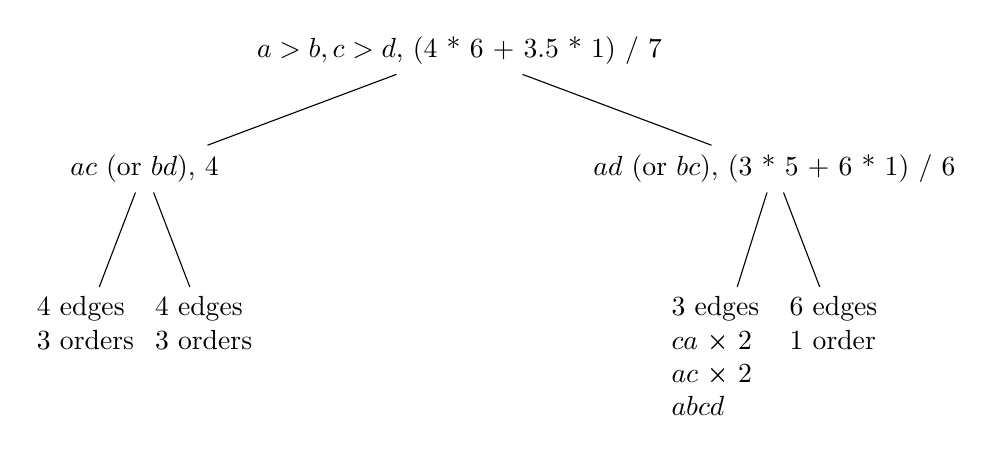
\begin{tikzpicture}
		\path (-10mm, -9mm) coordinate (offsetL);
		\path (10mm, -9mm) coordinate (offsetR);
		\path (0, -4mm) coordinate (offsetG);
		\path [sibling distance = 8cm, level 2/.style = {sibling distance = 1.5cm, align = left, anchor = north}] node[anchor=north] {$a > b, c > d$, \esp{(4 * 6 + 3.5 * 1) / 7}}
			child {
				node {$a \relq c$ (or $b \relq d$), \esp{4}}
				child {
					node {
						4 edges\\
						3 orders
					}
				}
				child {
					node {
						4 edges\\
						3 orders
					}
				}
			}
			child {
				node {$a \relq d$ (or $b \relq c$), \esp{(3 * 5 + 6 * 1) / 6}}
				child {
					node {
						3 edges\\
						$ca$ × 2\\
						$ac$ × 2\\
						$abcd$
					}
				}
				child {
					node {
						6 edges\\
						1 order
					}
				}
			}
		;
	\end{tikzpicture}
	\caption{The case $m = 4$, three questions, continued.}
	\label{fig:m4Cont}
\end{figure}

%\bibliography{bibl}

\section{Example context}
$N$ the voters (reviewers), $\card{N} = n$; $X$ the items (articles submitted to a conference), $\card{X} = m$. $PO(X)$ the partially ordered sets over $X$. Let $Q \in PO(X)^N$ represent some partial knowledge of the voters preferences. Consider $f: PO(X)^N → \powersetz{X}$ an enlarged voting rule, that selects winning items on the basis of partial knowledge of the preferences of the voters. Define $f(Q) = \min_{x \in X} \max_{y \in X, (>_{i \in N}) \in compl(Q)} s(y, (>_{i \in N})) - s(x, (>_{i \in N}))$ as selecting the alternatives that minimize the worst regret, where $s$ is the Borda scoring rule (attributing to an alternative at a profile as many points as that alternative beats other alternatives, summed over all voters).

We are interested in asking questions so as to let the regret diminish as fast as possible.
\end{document}

